\subsection*{A. Reproduksi}
\begin{verbatim}
pip install -r kode/requirements.txt
python -m pytest -q kode/tests
python kode/run_all.py --task all --mode train
python kode/run_all.py --task t1 --mode reproduce
\end{verbatim}
Perintah ketiga menghasilkan semua angka, gambar, tabel, dan tiga file prediksi; perintah keempat mereproduksi
angka kunci dari model tersimpan dalam kurang dari satu menit. Seed 42. Versi library tercatat di setiap \url{kode/outputs/results/*.json}. Seluruh angka laporan berasal dari
\url{kode/outputs/tables/angka.tex} yang dibuat otomatis dari file hasil.

\subsection*{B. Penggunaan AI}
Kode disusun dengan bantuan Claude (Anthropic). Kelompok memverifikasi hasilnya dengan tes otomatis (metrik dan anti-kebocoran fitur),
membandingkan skema validasi, menjalankan ulang \texttt{-{}-mode reproduce}, dan memeriksa setiap tabel serta gambar. Rincian per anggota ada di \texttt{kontribusi.md}.

\subsection*{C. Tabel dan gambar tambahan}
\begin{figure}[H]\centering
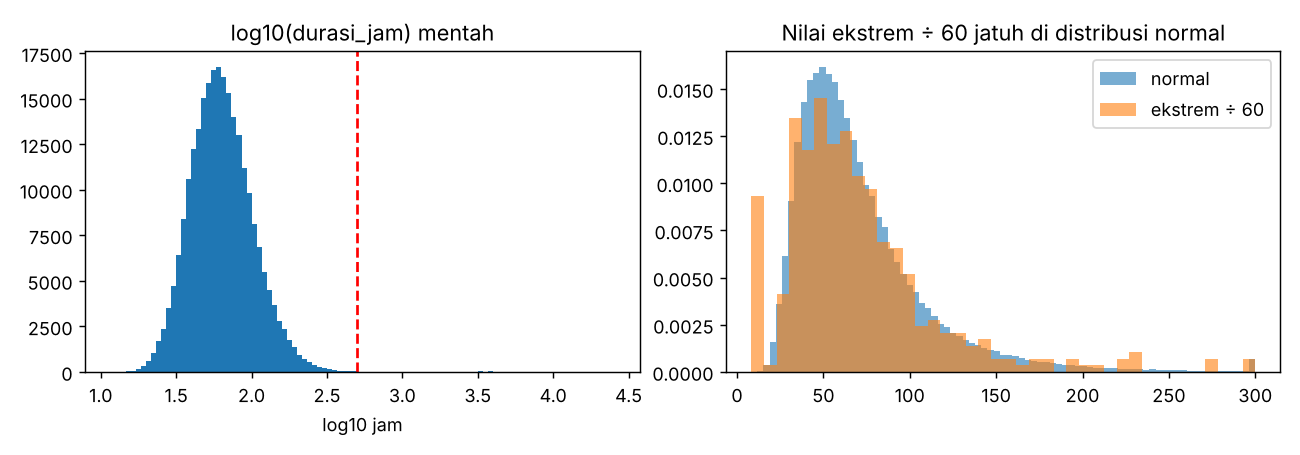
\includegraphics[width=.85\linewidth]{t1_audit_durasi.png}
\caption{Tugas 1: durasi ekstrem (> 500 jam) setelah dibagi 60 jatuh di distribusi normal.}\label{fig:t1durasi}
\end{figure}
\begin{table}[ht]
\centering\small
\resizebox{\ifdim\width>\linewidth\linewidth\else\width\fi}{!}{%
\begin{tabular}{lrrrr}
\toprule
fitur & KS & Spearman & mean\_train & mean\_test \\
\midrule
jumlah\_scan & 0.915 & 0.771 & 9.651 & 1.502 \\
antrean\_hub\_asal & 0.263 & 0.177 & 3328.677 & 4618.876 \\
f30 & 0.232 & -0.004 & 0.497 & 1.092 \\
f17 & 0.108 & 0.215 & 0.264 & 0.346 \\
f35 & 0.092 & 0.106 & 1.006 & 1.029 \\
hujan\_tujuan\_mm & 0.036 & 0.031 & 7.998 & 7.307 \\
hujan\_asal\_mm & 0.033 & 0.019 & 7.925 & 7.289 \\
f24 & 0.010 & 0.001 & 0.004 & -0.008 \\
\bottomrule
\end{tabular}
}
\caption{Fitur dengan beda distribusi train–test terbesar (KS) dan korelasi Spearman dengan durasi.}
\label{tab:t1_audit_ks}
\end{table}

\begin{table}[ht]
\centering\small
\begin{tabular}{lrrr}
\toprule
perlakuan & pinball50 & pinball90 & coverage90 \\
\midrule
bagi60 & 6.853 & 4.349 & 0.875 \\
buang & 6.851 & 4.354 & 0.873 \\
biarkan & 6.924 & 4.376 & 0.877 \\
\bottomrule
\end{tabular}
\caption{Perlakuan durasi ekstrem (> 500 jam), dievaluasi pada label yang sudah dikoreksi.}
\label{tab:t1_audit_target}
\end{table}

\begin{table}[ht]
\centering\small
\resizebox{\ifdim\width>\linewidth\linewidth\else\width\fi}{!}{%
\begin{tabular}{rrrrr}
\toprule
cfg & pinball50 & pinball90 & coverage90 & skor \\
\midrule
0 & 6.824 & 4.282 & 0.890 & 11.106 \\
1 & 6.832 & 4.271 & 0.895 & 11.103 \\
2 & 6.808 & 4.335 & 0.885 & 11.143 \\
3 & 6.768 & 4.286 & 0.891 & 11.054 \\
4 & 6.757 & 4.326 & 0.882 & 11.084 \\
\bottomrule
\end{tabular}
}
\caption{Tuning LightGBM pada fold waktu (skor = pinball50 + pinball90).}
\label{tab:t1_tuning}
\end{table}

\begin{table}[ht]
\centering\small
\resizebox{\ifdim\width>\linewidth\linewidth\else\width\fi}{!}{%
\begin{tabular}{lrrrrrr}
\toprule
mitra\_kurir & n & median\_durasi & pinball50 & pinball90 & coverage90 & mae \\
\midrule
K07 & 5448 & 77.800 & 10.236 & 5.327 & 0.806 & 20.473 \\
K02 & 8309 & 66.200 & 6.901 & 4.328 & 0.921 & 13.802 \\
K03 & 7621 & 64.800 & 6.837 & 4.372 & 0.921 & 13.674 \\
K10 & 4179 & 63.000 & 6.779 & 4.399 & 0.928 & 13.558 \\
K12 & 2808 & 62.500 & 6.692 & 4.232 & 0.927 & 13.384 \\
K06 & 5403 & 62.800 & 6.638 & 4.420 & 0.934 & 13.277 \\
K05 & 6197 & 62.900 & 6.516 & 4.115 & 0.931 & 13.032 \\
K04 & 6777 & 59.700 & 6.344 & 4.215 & 0.941 & 12.688 \\
K11 & 3392 & 60.800 & 6.308 & 4.114 & 0.938 & 12.615 \\
K09 & 4072 & 58.500 & 6.273 & 4.298 & 0.938 & 12.546 \\
K01 & 9621 & 57.700 & 6.211 & 4.086 & 0.943 & 12.423 \\
K08 & 4777 & 52.300 & 5.866 & 3.955 & 0.957 & 11.732 \\
\bottomrule
\end{tabular}
}
\caption{Error per mitra\_kurir (fold F2, model final + kalibrasi).}
\label{tab:t1_breakdown_mitra_kurir}
\end{table}

\begin{table}[ht]
\centering\small
\begin{tabular}{lr}
\toprule
fitur & mean |SHAP| \\
\midrule
layanan & 11.504 \\
jarak\_km & 8.954 \\
kota\_tujuan\_te & 5.972 \\
f17 & 3.789 \\
f04 & 3.449 \\
antrean\_hub\_asal & 2.671 \\
f35 & 2.450 \\
pulau\_tujuan & 2.060 \\
kota\_asal\_te & 2.017 \\
cod & 2.004 \\
\bottomrule
\end{tabular}
\caption{Rata-rata |SHAP| model P50 (3.000 sampel validasi).}
\label{tab:t1_shap}
\end{table}

\begin{table}[ht]
\centering\small
\resizebox{\ifdim\width>\linewidth\linewidth\else\width\fi}{!}{%
\begin{tabular}{llrrr}
\toprule
skema & fold & pr\_auc & roc\_auc & n\_fraud \\
\midrule
waktu & F1 & 0.792 & 0.988 & 666 \\
waktu & F2 & 0.781 & 0.991 & 640 \\
random & R1 & 0.827 & 0.989 & 793 \\
random & R2 & 0.816 & 0.988 & 792 \\
random & R3 & 0.829 & 0.994 & 792 \\
\bottomrule
\end{tabular}
}
\caption{Validasi berbasis waktu (label matang) vs random stratified 3-fold.}
\label{tab:t2_validasi}
\end{table}

\begin{table}[ht]
\centering\small
\begin{tabular}{lr}
\toprule
fitur & porsi gain \\
\midrule
perangkat\_baru & 0.097 \\
menit\_sejak\_trx\_terakhir & 0.076 \\
m\_trx\_7h & 0.075 \\
nominal & 0.067 \\
kategori\_merchant & 0.057 \\
trx\_1j & 0.057 \\
refund\_merchant\_30h & 0.050 \\
persen\_saldo & 0.046 \\
umur\_akun\_hari & 0.037 \\
gagal\_login\_24j & 0.034 \\
\bottomrule
\end{tabular}
\caption{10 fitur terpenting (gain) model F2.}
\label{tab:t2_importance}
\end{table}

\begin{table}[ht]
\centering\small
\resizebox{\ifdim\width>\linewidth\linewidth\else\width\fi}{!}{%
\begin{tabular}{lrrrrrrrrr}
\toprule
kategori\_merchant & n & n\_fraud & rate\_fraud\_\% & pr\_auc & recall & FN & FP & nominal\_FN\_juta & biaya\_juta \\
\midrule
elektronik & 11007 & 93 & 0.84 & 0.78 & 0.83 & 16 & 263 & 11.21 & 19.71 \\
fashion & 6992 & 50 & 0.72 & 0.29 & 0.36 & 32 & 90 & 9.21 & 11.91 \\
gadget & 4262 & 78 & 1.83 & 0.82 & 0.92 & 6 & 155 & 3.24 & 8.91 \\
kecantikan & 4439 & 29 & 0.65 & 0.20 & 0.17 & 24 & 56 & 4.96 & 6.49 \\
voucher\_game & 4830 & 106 & 2.19 & 0.91 & 0.79 & 22 & 19 & 1.19 & 3.77 \\
emas & 1611 & 39 & 2.42 & 0.85 & 0.97 & 1 & 91 & 0.12 & 3.35 \\
toko\_online & 8267 & 64 & 0.77 & 0.83 & 0.47 & 34 & 30 & 1.67 & 3.17 \\
top\_up\_ewallet & 5325 & 59 & 1.11 & 0.94 & 0.92 & 5 & 30 & 0.96 & 3.06 \\
pulsa\_data & 9648 & 73 & 0.76 & 0.87 & 0.48 & 38 & 7 & 0.66 & 1.71 \\
rumah\_tangga & 3959 & 5 & 0.13 & 0.56 & 0.60 & 2 & 2 & 0.93 & 1.05 \\
hotel & 3695 & 6 & 0.16 & 0.84 & 0.67 & 2 & 10 & 0.50 & 0.85 \\
makanan\_minuman & 15255 & 15 & 0.10 & 0.80 & 0.73 & 4 & 2 & 0.51 & 0.83 \\
\bottomrule
\end{tabular}
}
\caption{Error per kategori\_merchant (fold F2, aturan biaya).}
\label{tab:t2_breakdown_kategori_merchant}
\end{table}

\begin{table}[ht]
\centering\small
\begin{tabular}{lrrr}
\toprule
kelompok & n\_kolom & perubahan\_label\_\% & 1-ARI \\
\midrule
promo \& pembayaran & 4 & 22.121 & 0.482 \\
RFM \& nilai & 8 & 26.886 & 0.450 \\
perilaku pasca-beli & 3 & 24.887 & 0.448 \\
profil & 7 & 19.966 & 0.326 \\
aktivitas aplikasi & 5 & 17.017 & 0.279 \\
waktu belanja (CLR) & 4 & 10.419 & 0.249 \\
kategori (CLR) & 16 & 2.208 & 0.056 \\
\bottomrule
\end{tabular}
\caption{Kepentingan kelompok fitur: seberapa banyak label berubah jika kelompok diacak.}
\label{tab:t3_kepentingan_kelompok}
\end{table}

\begin{table}[ht]
\centering\small
\resizebox{\ifdim\width>\linewidth\linewidth\else\width\fi}{!}{%
\begin{tabular}{rrrrrrrr}
\toprule
k & silhouette & calinski\_harabasz & davies\_bouldin & bic\_gmm & stabilitas\_ARI & stabilitas\_std & ukuran\_terkecil\_\% \\
\midrule
2 & 0.494 & 3096.941 & 0.775 & -571761.578 & 1.000 & 0.000 & 5.613 \\
3 & 0.107 & 2109.214 & 2.399 & -609571.139 & 0.993 & 0.003 & 5.613 \\
4 & 0.092 & 1633.231 & 2.639 & -626828.831 & 0.984 & 0.006 & 5.613 \\
5 & 0.090 & 1352.417 & 2.692 & -640605.420 & 0.843 & 0.154 & 5.613 \\
6 & 0.089 & 1179.265 & 2.735 & -648559.025 & 0.655 & 0.178 & 5.613 \\
7 & 0.093 & 1079.320 & 2.494 & -697001.060 & 0.983 & 0.004 & 1.426 \\
8 & 0.092 & 977.446 & 2.544 & -697171.874 & 0.982 & 0.005 & 1.426 \\
9 & 0.082 & 832.486 & 3.112 & -707349.673 & 0.869 & 0.142 & 5.613 \\
10 & 0.087 & 809.407 & 2.818 & -694258.726 & 0.685 & 0.067 & 1.426 \\
11 & 0.082 & 751.211 & 2.815 & -734124.145 & 0.680 & 0.103 & 1.426 \\
12 & 0.083 & 697.923 & 2.946 & -728314.381 & 0.596 & 0.111 & 1.426 \\
\bottomrule
\end{tabular}
}
\caption{Kriteria jumlah cluster (K-Means). Stabilitas = rata-rata ARI antar 5 run subsampling 80\%.}
\label{tab:t3_kriteria_k}
\end{table}

\begin{table}[ht]
\centering\small
\begin{tabular}{rrr}
\toprule
cluster\_run\_acuan & ukuran & jaccard\_rata2 \\
\midrule
0 & 9767 & 0.972 \\
1 & 18337 & 0.989 \\
2 & 26618 & 0.990 \\
3 & 6736 & 1.000 \\
4 & 20200 & 0.979 \\
5 & 1711 & 1.000 \\
6 & 17049 & 0.992 \\
7 & 19582 & 0.990 \\
\bottomrule
\end{tabular}
\caption{Jaccard rata-rata tiap cluster terhadap cluster paling mirip di run lain.}
\label{tab:t3_jaccard}
\end{table}

\begin{figure}[H]\centering
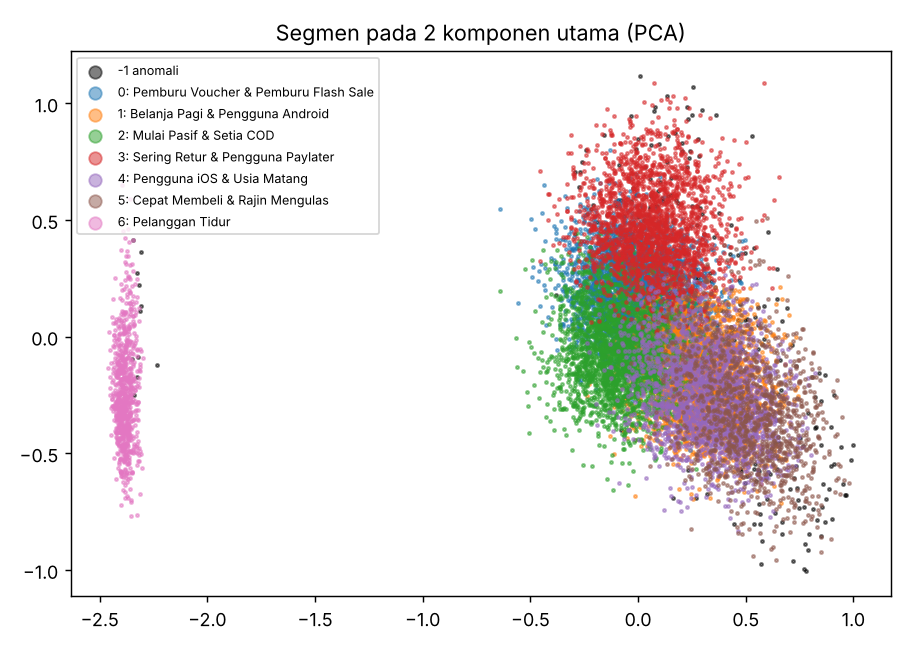
\includegraphics[width=.6\linewidth]{t3_pca.png}
\caption{Tugas 3: segmen pada dua komponen utama.}\label{fig:t3pca}
\end{figure}
